\documentclass[acmtog]{acmart}
\usepackage{graphicx}
\usepackage{subfigure}
\usepackage{natbib}
% Title portion
\title{Assignment 3 : Direct Lighting and Texturing} 
\author{Student Name Chenghua Yang \quad Student No. 2019533089 \quad Email yangchh@shanghaitech.edu.cn}

% Document starts
\begin{document}
\maketitle

\vspace*{2 ex}

\section{Introduction}
	\quad This time's homework realise a simple one-time-raytracing renderer.
	\\\quad The raytracing only generate ray direct from the camera and the 1st ray hit point, which is aim to rebuild the projection based render with phong lighting model.
	\\\quad I finished the essential part including the pihole-camera, the intersection algorithm, the phong lighting intergrator and the texture mapping.
	\\\quad Also I do the a simple optional part, the anti-aliasing with uniform multiple sample.

\section{Content}
	\subsection{The pinhole camera to generate rays.}
	\subsection{The intersection algorithm}
	\subsection{The texture mapping}
	\subsection{The integrator}

\section{Implementation Details}


\subsection{The pinhole camera to generate rays.}
\quad The pinhole camera shoot ray from a original point.\\\\
\quad Before we generate rays, firstly we should let the camera look at the right direction.\\
Given a lookat point and reference up direction, we can figure out the forward, up and right direction of the camera, thus to present its look-at direction.\\\\
\quad To shoot the ray ,we first fetch the number of the pixel (dx,dy), then convert it to the world spacepixel postion on the picture(or the screen). see Fig.1.\\
The essential part of this is to fix the fov and focal length to simplify the formula, then use the tan to find out the vertical/horizontal distance between center and the pixel. see Fig.2.
	\begin{figure}[h]
		\centering
		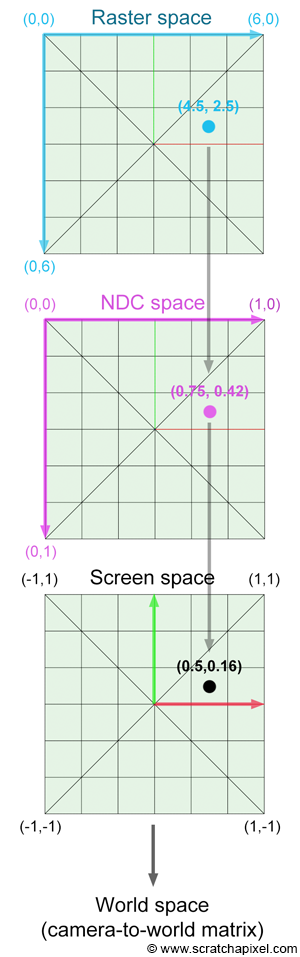
\includegraphics[width=5cm,height=15cm]{cambasic1A.png}
		\caption{The whole transform process}
	\end{figure}
	\begin{figure}[h]
		\centering
		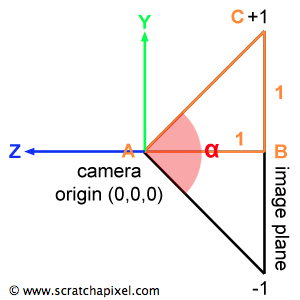
\includegraphics[width=5cm,height=5cm]{camprofile.png}
		\caption{from screen to world using alpha angle}
	\end{figure}
	
	
\subsection{The intersection algorithm}
\quad This time's raytracing homework nearly skips the intersection part which should be a mainly difficult part of raytracing, and replace it with the analystic geometry intersection.\\\\
\quad To interact with all the algorithm, the scene function intersect() simply iterate sequetially through every geometry in the scene.\\
\quad Then, with each geometry(sphere or parallegram), there is a solution of polynomial equation as $Point_{onRay}=Point_{onGeometry}$. This will be a quadratic equation in the sphere case. See Fig.3.
	\begin{figure}[h]
		\centering
		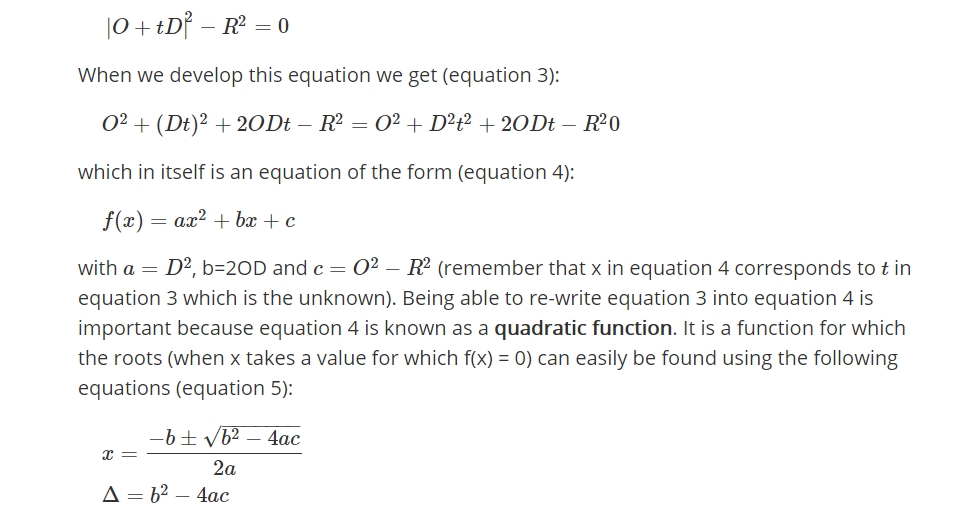
\includegraphics[width=7cm,height=4cm]{solve.png}
		\caption{the quadratic equation of the sphere intersection}
	\end{figure}


\subsection{The texture mapping}
\quad The texure mapping process including turn a world position on geomrtry into a uv position\\
and validate the uv, sample it from the texture.\\\\
\quad To map a position into uv, there will be several map to use. I choose to use the angle term directly, the phi angle represents the u and the theta angle represents the v. see Fig.4.\\\\
	\begin{figure}[h]
		\centering
		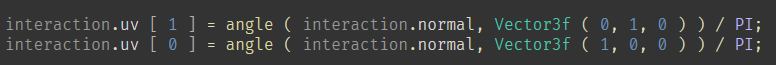
\includegraphics[width=8cm,height=0.5cm]{map.png}
		\caption{the sphere coordinate map to uv}
	\end{figure}
\quad To sample a pixel on the texture, we need to specify the uv wrap mode because the original uv coordinate may out of [0,1]x[0,1] and thus invalid. Also we need to specify the pixel interpolation mode, to make the image more smooth on texture edge.\\
\quad Here I choose the repeart mode the the linear interpolation.\\
The repeat mode uv wrap need a saw wave as the original signal and to strech this wave in time and amplitude we will get the repeat function. See Fig.5.\\
 	\begin{figure}[h]
		\centering
		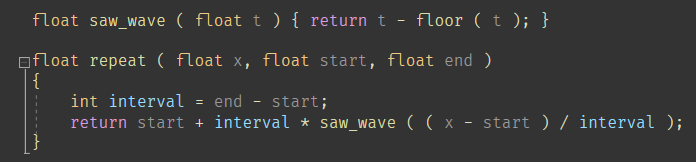
\includegraphics[width=8cm,height=2cm]{repeat.png}
		\caption{The repeat wrap implementation}
	\end{figure}
The linear interpolation simply choose the 4 pixel around the uv postion and interpolate them according to the distance between each pixel position and the real uv pixel position.\\\\
\quad There is one problem that make me confused. When the generate-checkboard using odd num-chekers arg, the texture will present line of aliasing in the image, the problem might be related to the interpolation.
\subsection{The integrator}
\quad The integrator is the another main algorithm of this program.The integrator part is in charge of calculate the randiance of every ray and assign them to pixel to render a image.
To generate the picuture, the intergrator generate rays from the camera point accroding to the pixel position on the image. Every pixel may use multiple rays to do the anti-aliasing.\\\\
A ray may intersects with nothing or the light or a geometry. In the first 2 case, the radiance of the ray is just black or the color of light. The 3rd case is the main problem the algorithm solves.
In normal raytracing,the ray which intersect with a reflection object need to recursively generate rays again to integrate the randiance of the ray its own. However, here we simply replace the deeper ray tracing with the phong lighting model. The model tells us that a randiance of a given point on the algorithm can be calculated by the light source, the vision direction and the point info.\\
In general, the phong lighting model use the input: the ray , the intersection info, the light sources to generate the output: the radiance of this ray.\\
The phong model have been conclude from my previous homework report. However, these are still several important things to say:\\
\quad\quad	1. The randiance of the original ray is determined by all the light source. More specifically, we need to generate every second ray for every light sources, if the second ray can reach the light source directly without being blocked, the light source's randiance will be considered.\\
\quad\quad	2. The specular and diffuse part shouldn't be divided by the distance square.
\section{Results}
With all the algorithms above, we now are able to generate one image represent the 1st and 0nd reflections light rays of a given scene. See Fig.6 for config 11.
\begin{figure}[h]
		\centering
		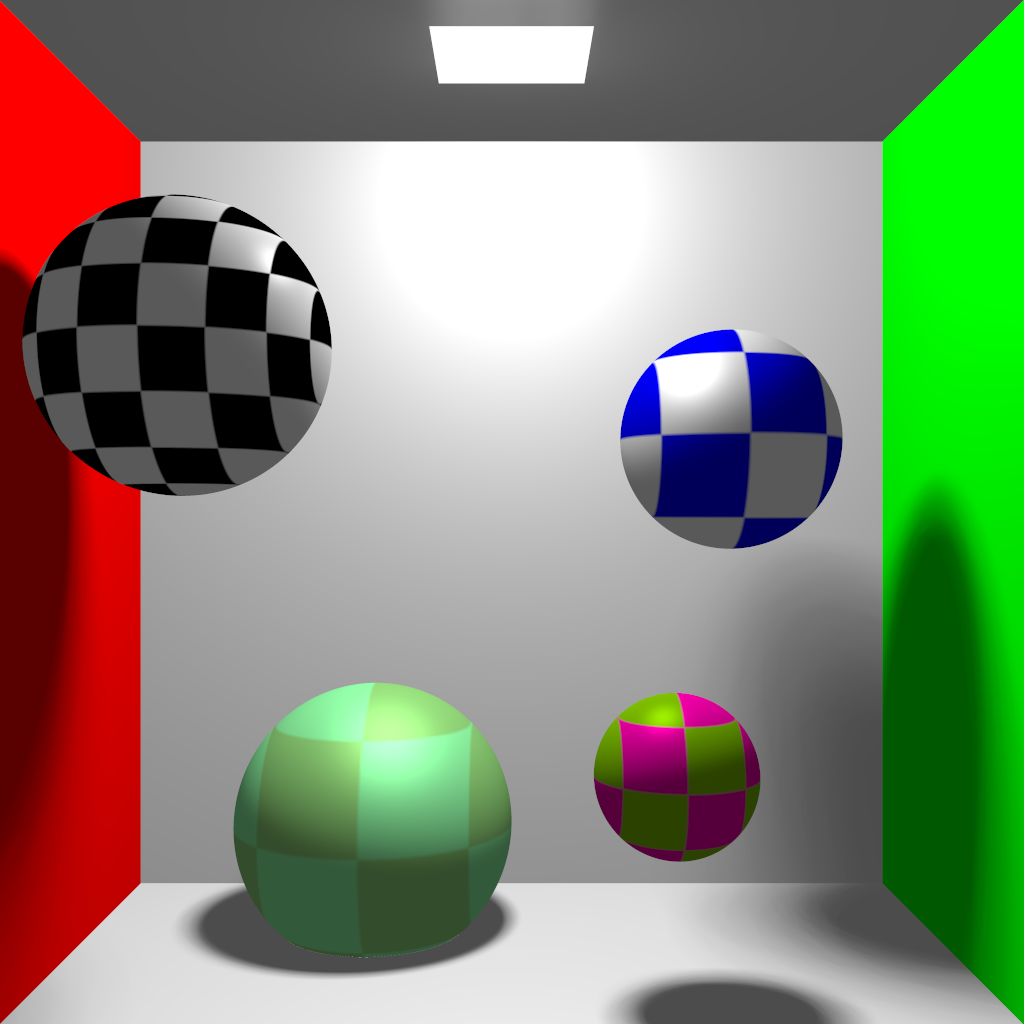
\includegraphics[width=8cm,height=8cm]{output11_final.png}
		\caption{The final result of config11, 1024x1024 resolution and 4X anti-aliasing}
	\end{figure}

\section{Conclusion}
This assignment helps me to make the concept of ray-tracing clear and gives me a comprehensive experience of how to realise a whole program of ray-tracing, which is about Object design, Multi-thread, image sampling and so on.

\end{document}
